\iffalse
\chapter{2022}
\author{EE24BTECH11040}
\section{ph}
\fi

\item A parallel plate capacitor with spacing $d$ and area of cross-section $A$ is connected to a source of voltage $V$. If the plates are pulled apart quasistatically to a spacing
of 2$d$, then which of the following statements are correct? 

\begin{enumerate}
\item The force between the plates at spacing $2d$ is $\frac{1}{8}\brak{\frac{\epsilon_0AV^2}{d^2}}$
\item The work done in moving the plates is $\frac{1}{8}\brak{\frac{\epsilon_0AV^2}{d}}$
\item The energy transferred to the voltage source is $\frac{1}{2}\brak{\frac{\epsilon_0AV^2}{d}}$
\item The energy of the capacitor reduces by $\frac{1}{4}\brak{\frac{\epsilon_0AV^2}{d}}$
\end{enumerate}

\item A system with time independent Hamiltonian $H(q,p)$ has two constants of motion $f(q,p)$ and $g(q,p)$. Then which of the following Poisson brackets are always zero?

\begin{enumerate}
\item $\cbrak{H,f+g}$
\item $\cbrak{H,{f,g}}$
\item $\cbrak{H+f,g}$
\item $\cbrak{H,H+fg}$
\end{enumerate}

\item In the action-angle variables $(I_1,I_2,\theta_1,\theta_2)$, consider the Hamiltonian $H=4I_1I_2$ and $0\leq\theta_1,\theta_2<2\pi$. Let $\frac{I_1}{I_2}=\frac{1}{2}$. Which of the following are possible plots of the trajectories with different initial conditions in $\theta_1-\theta_2$ plane?

\begin{enumerate}
\item 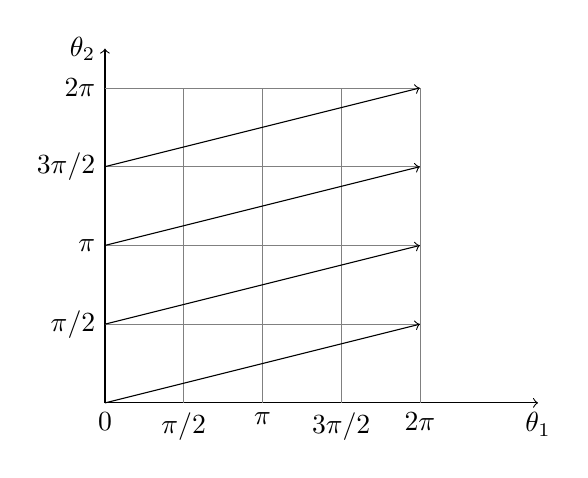
\begin{tikzpicture}
    \draw[->] (0,0) -- (5.5,0) node[below] {$\theta_1$};
    \draw[->] (0,0) -- (0,4.5) node[left] {$\theta_2$};
    \foreach \x in {1,2,3,4} {
        \draw[gray, very thin] (\x,0) -- (\x,4);
    }
    \foreach \y in {1,2,3,4} {
        \draw[gray, very thin] (0,\y) -- (4,\y);
    }
    \node[below] at (0,0) {$0$};
    \node[below] at (1,0) {$\pi/2$};
    \node[below] at (2,0) {$\pi$};
    \node[below] at (3,0) {$3\pi/2$};
    \node[below] at (4,0) {$2\pi$};
    \node[left] at (0,1) {$\pi/2$};
    \node[left] at (0,2) {$\pi$};
    \node[left] at (0,3) {$3\pi/2$};
    \node[left] at (0,4) {$2\pi$};
    \draw[->] (0,0) -- (4,1);
    \draw[->] (0,1) -- (4,2);
    \draw[->] (0,2) -- (4,3);
    \draw[->] (0,3) -- (4,4);
\end{tikzpicture}
\item 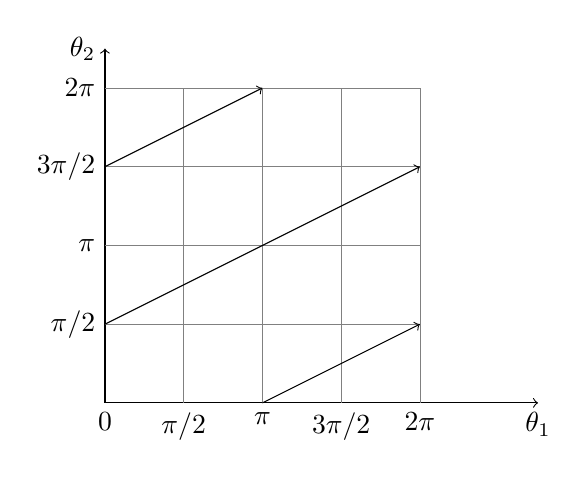
\begin{tikzpicture}
    \draw[->] (0,0) -- (5.5,0) node[below] {$\theta_1$};
    \draw[->] (0,0) -- (0,4.5) node[left] {$\theta_2$};

    \foreach \x in {1,2,3,4} {
        \draw[gray, very thin] (\x,0) -- (\x,4);
    }
    \foreach \y in {1,2,3,4} {
        \draw[gray, very thin] (0,\y) -- (4,\y);
    }

    \node[below] at (0,0) {$0$};
    \node[below] at (1,0) {$\pi/2$};
    \node[below] at (2,0) {$\pi$};
    \node[below] at (3,0) {$3\pi/2$};
    \node[below] at (4,0) {$2\pi$};
    \node[left] at (0,1) {$\pi/2$};
    \node[left] at (0,2) {$\pi$};
    \node[left] at (0,3) {$3\pi/2$};
    \node[left] at (0,4) {$2\pi$};

    \draw[->] (0,3) -- (2,4);
    \draw[->] (0,1) -- (4,3);
    \draw[->] (2,0) -- (4,1);
\end{tikzpicture}
\item 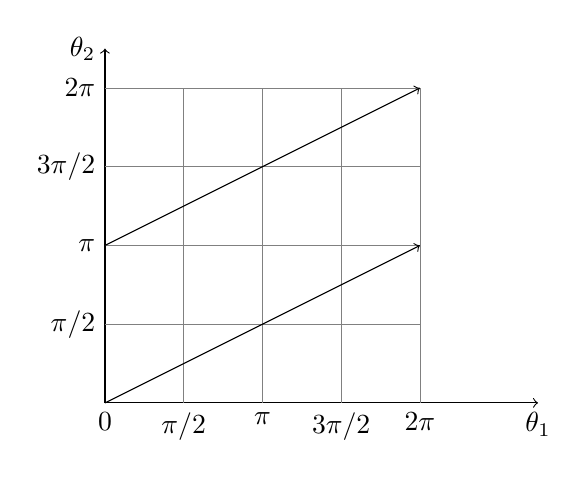
\begin{tikzpicture}
    \draw[->] (0,0) -- (5.5,0) node[below] {$\theta_1$};
    \draw[->] (0,0) -- (0,4.5) node[left] {$\theta_2$};

    \foreach \x in {1,2,3,4} {
        \draw[gray, very thin] (\x,0) -- (\x,4);
    }
    \foreach \y in {1,2,3,4} {
        \draw[gray, very thin] (0,\y) -- (4,\y);
    }

    \node[below] at (0,0) {$0$};
    \node[below] at (1,0) {$\pi/2$};
    \node[below] at (2,0) {$\pi$};
    \node[below] at (3,0) {$3\pi/2$};
    \node[below] at (4,0) {$2\pi$};
    \node[left] at (0,1) {$\pi/2$};
    \node[left] at (0,2) {$\pi$};
    \node[left] at (0,3) {$3\pi/2$};
    \node[left] at (0,4) {$2\pi$};

    \draw[->] (0,2) -- (4,4);
    \draw[->] (0,0) -- (4,2);
\end{tikzpicture}
\item 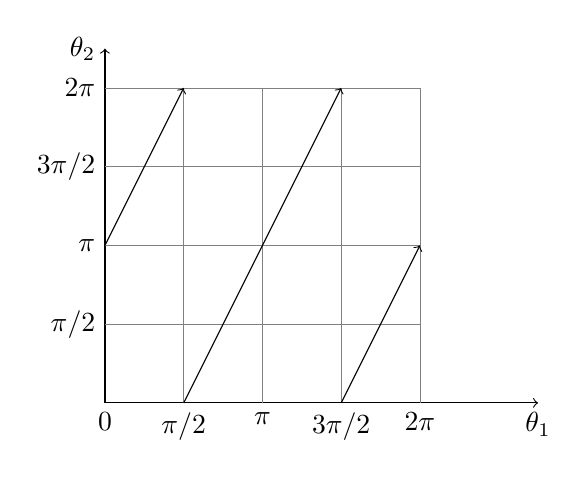
\begin{tikzpicture}
    \draw[->] (0,0) -- (5.5,0) node[below] {$\theta_1$};
    \draw[->] (0,0) -- (0,4.5) node[left] {$\theta_2$};

    \foreach \x in {1,2,3,4} {
        \draw[gray, very thin] (\x,0) -- (\x,4);
    }
    \foreach \y in {1,2,3,4} {
        \draw[gray, very thin] (0,\y) -- (4,\y);
    }

    \node[below] at (0,0) {$0$};
    \node[below] at (1,0) {$\pi/2$};
    \node[below] at (2,0) {$\pi$};
    \node[below] at (3,0) {$3\pi/2$};
    \node[below] at (4,0) {$2\pi$};
    \node[left] at (0,1) {$\pi/2$};
    \node[left] at (0,2) {$\pi$};
    \node[left] at (0,3) {$3\pi/2$};
    \node[left] at (0,4) {$2\pi$};

    \draw[->] (0,2) -- (1,4);
    \draw[->] (1,0) -- (3,4);
    \draw[->] (3,0) -- (4,2);
\end{tikzpicture}
\end{enumerate}

\item A particle of mass m in the $x-y$ plane is confined in an infinite two-dimensional well with vertices at $(0,0)$, $(0,L)$, $(L,L)$, $(L,0)$. The eigenfunctions of this particle are $\psi_{n_x,n_y} = \frac{2}{L}\sin{\brak{\frac{n_x\pi x}{L}}}\sin{\brak{\frac{n_y\pi y}{L}}}$. If perturbation of the form $V=Cxy$, where $C$ is a real constant, is applied, then which of the following statements are correct for the first excited state?

\begin{enumerate}
\item The unperturbed energy is $\frac{3\pi^2h^2}{2mL^2}$
\item The unperturbed energy is $\frac{5\pi^2h^2}{2mL^2}$
\item First order energy shift due to the applied perturbation is zero
\item The shift $(\delta)$ in energy due to the applied perturbation is determined by an equation of the form $\begin{vmatrix}
a-\delta & b \\
b & a-\delta
\end{vmatrix}$
$=0$, where $a$ and $b$ are real, non-zero constants
\end{enumerate}

\item A junction is formed between a metal on the left and an $n$-type semiconductor on the right. Before forming the junction, the Fermi level $E_F$ of the metal lies below that of the semiconductor. Then which of the following schematics are correct for the bands and the $I-V$ characteristics of the junction?

\begin{enumerate}
\item 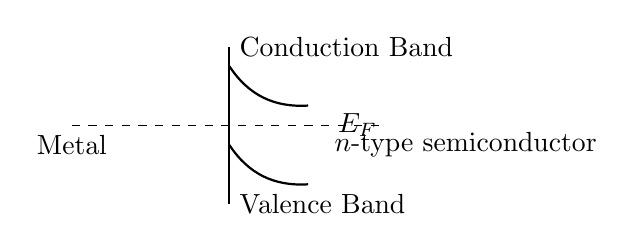
\begin{tikzpicture}
    \draw[dashed] (-2,0) -- (2,0) node[left] {$E_F$};
    \node at (-2,-0.25) {Metal};
    \node at (3,-0.25) {$n$-type semiconductor};
    \draw[thick] (0,0) -- ++(0,1) node[right] {Conduction Band};
    \draw[thick] (0,0) -- ++(0,-1) node[right] {Valence Band};
    \draw[thick] (0,0.75) to[bend right=30] (1,0.25);
    \draw[thick] (0,-0.25) to[bend right=30] (1,-0.75);
\end{tikzpicture}
\item 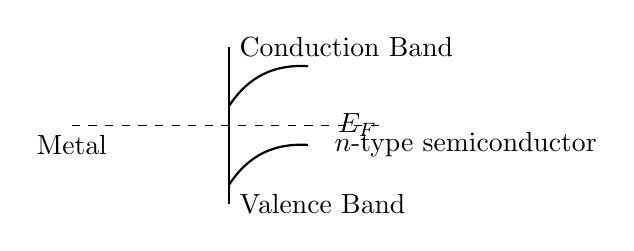
\begin{tikzpicture}
    \draw[dashed] (-2,0) -- (2,0) node[left] {$E_F$};
    \node at (-2,-0.25) {Metal};
    \node at (3,-0.25) {$n$-type semiconductor};
    \draw[thick] (0,0) -- ++(0,1) node[right] {Conduction Band};
    \draw[thick] (0,0) -- ++(0,-1) node[right] {Valence Band};
    \draw[thick] (0,0.25) to[bend left=30] (1,0.75);
    \draw[thick] (0,-0.75) to[bend left=30] (1,-0.25);
\end{tikzpicture}
\item \begin{tikzpicture}
    \draw[->] (-3,0) -- (3,0) node[right] {$V$};
    \draw[->] (0,-2) -- (0,3) node[above] {$I$};
    \draw (-2.5,0) -- (-1.5,0) node[above] {$-V_0$};
    \draw[thick] (-2.5,-0.2) -- (-0.2,-0.2) to[bend right] (2,2.5);
\end{tikzpicture}
\item \begin{tikzpicture}
    \draw[->] (-3,0) -- (3,0) node[right] {$V$};
    \draw[->] (0,-2) -- (0,3) node[above] {$I$};
    \draw (-2.5,0) -- (-1.5,0) node[above] {$-V_0$};
    \draw[thick] (-2,-1) --  (0,0) to[bend right] (2,2.5);
\end{tikzpicture}
\end{enumerate}

\item A plane polarized electromagnetic wave propagating in $y-z$ plane is incident at the interface of two media at Brewster's angle. Taking $z=0$ as the boundary between the two media, the electric field of the reflected wave is given by
$$\vec{E_R} = A_R \cos{\sbrak{k_0\cbrak{\frac{\sqrt{3}}{2}y - \frac{1}{2}z}-\omega t}}\hat{x}$$
then which among the following statements are correct?

\begin{enumerate}
\item The angle of refraction is $\frac{\pi}{6}$
\item Ratio of permittivity of the medium of refraction ($\epsilon_2$) with respect to the medium on incidence ($\epsilon_1$), $\frac{\epsilon_2}{\epsilon_1}=3$
\item The incident wave can have components of its electric field in $y-z$ plane
\item The angle of reflection is $\frac{\pi}{6}$
\end{enumerate}

\item The minimum number of two-input NAND gates required to implement the following Boolean expression is \_
$$Y = \sbrak{A\bar{B} \brak{C + BD} + \bar{A}\bar{B}}C$$

\item In a nucleus, the interaction $V_{so}\vec{l}\cdot\vec{s}$ is responsible for creating spin-orbit doublets. The energy difference between $p_{\frac{1}{2}}$ and $p_{\frac{3}{2}}$ states in units of $V_{so}\frac{h^2}{2}$ is \_ (round off to the nearest integer)

\item Two identical particles of rest mass $m_0$ approach each other with equal and opposite velocity $v=0.5c$, where $c$ is the speed of light. The total energy of one particle as measured in the rest frame of the other is $E=\alpha m_0c^2$. The value of $\alpha$ is \_ (Round off to two decimal places)

\item In an X-Ray diffraction experiment on a solid with FCC structure, five diffraction peaks corresponding to (111), (200), (220), (311) and (222) planes are observed using 1.54\,\AA X-rays. On using 3\,\AA X-rays on the same solid, the number of observed peaks will be \_

\item For 1 mole of Nitrogen gas, the ratio $\brak{\frac{\Delta S_I}{\Delta S_{II}}}$ of entropy change of the gas in processes (I) and (II) mentioned below is \_ (Round off to one decimal place)
\\
(I) The gas is held at 1 atm and is cooled from 300 K to 77 K.
\\
(II) The gas is liquified at 77 K.
\\
(Take $C_p$ = 7.0 cal $\mathrm{mol}^{-1}$$\mathrm{K}^{-1}$, Latent heat $L$ = 1293.6 cal $\mathrm{mol}^{-1}$)

\item Frequency bandwidth $\Delta v$ of a gas laser of frequency $\nu$ Hz is 
$$\Delta v = \frac{2\nu}{c} \sqrt{\frac{\alpha}{A}}$$
where $\alpha = 3.44 \times 10^6 \mathrm{m}^{2} \mathrm{s}^{-2}$ at room temperature and $A$ is the atomic mass of the lasing atom. For ${}^{4}He$ - ${}^{20}Ne$ laser (wavelength = 633 nm), $\Delta v = n \times 10^9$ Hz. The value of $n$ is \_ (Round off to one decimal place) 

\item A current of 1 A is flowing through a very long solenoid made of winding density 3000 turns/m. As shown in the figure, a parallel plate capacitor, with plates oriented parallel to the solenoid axis and carrying surface charge density $6\epsilon_0C\mathrm{m}^{-2}$, is placed at the middle of the solenoid. The momentum density of the electromagnetic field at the midpoint X of the capacitor is $n \times 10^{13}$ N s $\mathrm{m}^{-3}$. The value of $n$ is \_ (Round off to the nearest integer). 
\\ (speed of light $c = 3 \times 10^8 \mathrm{ms}^{-1}$)

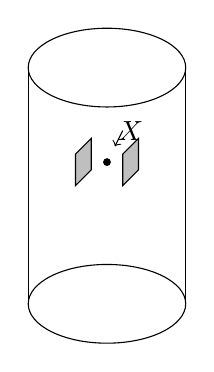
\begin{tikzpicture}
    \draw (0,0) ellipse (1 and 0.5);
    \draw (0,3) ellipse (1 and 0.5);
    \draw (1,0) -- (1,3);
    \draw (-1,0) -- (-1,3);
    \filldraw[fill=gray!50] (0.2,1.5) -- (0.4,1.7) -- (0.4,2.1) -- (0.2,1.9) -- cycle;
    \filldraw[fill=gray!50] (-0.2,1.7) -- (-0.4,1.5) -- (-0.4,1.9) -- (-0.2,2.1) -- cycle;
    \node[circle, fill=black, inner sep=1pt] at (0,1.8) {};

    % Label
    \node at (0.3,2.2) {$X$};
    \draw[->] (0.2,2.2) -- (0.1,2);
\end{tikzpicture}
